\documentclass{article}
\usepackage{amsmath,amssymb}
\usepackage{tikz}
\usetikzlibrary{arrows.meta,positioning,calc,shapes.geometric}
\pagestyle{empty}
\begin{document}
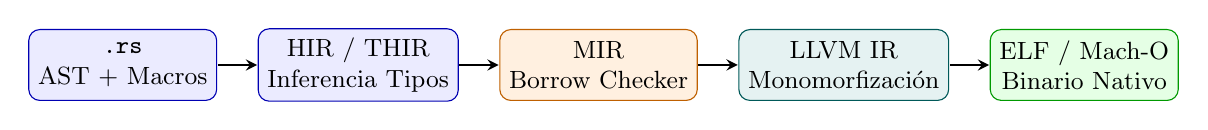
\begin{tikzpicture}
\tikzset{node distance=1.6cm, >=stealth, thick, font=\small}
\node[draw=blue!70!black, fill=blue!8, rounded corners, minimum width=2.2cm, minimum height=0.9cm, align=center] (src) {\texttt{.rs}\\AST + Macros};
\node[draw=blue!70!black, fill=blue!8, rounded corners, minimum width=2.2cm, minimum height=0.9cm, align=center, right=0.5cm of src] (hir) {HIR / THIR\\Inferencia Tipos};
\node[draw=orange!75!black, fill=orange!12, rounded corners, minimum width=2.5cm, minimum height=0.9cm, align=center, right=0.5cm of hir] (mir) {MIR\\Borrow Checker};
\node[draw=teal!70!black, fill=teal!10, rounded corners, minimum width=2.3cm, minimum height=0.9cm, align=center, right=0.5cm of mir] (llvm) {LLVM IR\\Monomorfización};
\node[draw=green!60!black, fill=green!10, rounded corners, minimum width=2.1cm, minimum height=0.9cm, align=center, right=0.5cm of llvm] (bin) {ELF / Mach-O\\Binario Nativo};
\draw[->] (src) -- (hir);
\draw[->] (hir) -- (mir);
\draw[->] (mir) -- (llvm);
\draw[->] (llvm) -- (bin);
\end{tikzpicture}
\end{document}
